\documentclass[a4paper,12pt]{article} % Можно заменить на report, если документ объемный

% Подключение пакетов
\usepackage[utf8]{inputenc}   % Поддержка UTF-8
\usepackage[russian]{babel}   % Русский язык
\usepackage{geometry}         % Настройки полей страницы
\geometry{a4paper, left=30mm, right=15mm, top=20mm, bottom=20mm}

\usepackage{setspace}         % Управление интервалами
\onehalfspacing               % Полуторный интервал

\usepackage{indentfirst}      % Красная строка в первом абзаце

\usepackage{graphicx}         % Работа с картинками
\usepackage{amsmath, amssymb} % Математические символы
\usepackage{graphicx} % Работа с изображениями
\usepackage[acronym]{glossaries}
\makeglossaries

\newacronym{gui}{GUI}{Graphical User Interface}

% Заголовок документа
\title{Пояснительная записка к дипломному проекту "Разработка desktop-приложения для учёта месторасположения вещей в пространстве хранения"}
\author{Белградская Елена Валерьевна}
\date{\today}

\begin{document}

\maketitle

\section*{Введение}
Организация хранения вещей в каком-либо пространстве, будь то склад, гараж, квартира и т.д. не простая задача. 
Особенно сложно эффективно реализовывать такую задачу, если нет удобного, визуализированного 
представления месторасположения уже имеющихся вещей в пространстве хранения.  
Если рассмотреть организацию хранения вещей в квартире, то можно предположить не редской ситуацию, когда сложно вспомнить, выкинута или нет та или иная вещь. Человек забыл, где точно хранилась эта вещь, предполагаемые места 
хранения проверить на наличие или отсутствие вещи представляется проблематичным по тем или иным причинам. 
Если рассматривать учёт хранения товаров на складе, то важность строгого учета месторасположения, количества и т.д. товаров на складе очевидна.
В то время, как приложений для учета хранения товаров на складе достаточно много, то удобных приложений для учета хранения вещей в "небольших" пространствах таких как квартиры, дачного дома, гаража и т.д. не много.
В связи с этим разработка приложения для учёта месторасположения вещей в пространстве хранения представляется целесообразной задачей.
\par
Целью данной дипломной работы является "Разработка desktop-приложения для учёта месторасположения вещей в пространстве хранения".
\\
Для достижения поставленной цели необходимо выполнить следующие задачи:

\begin{itemize}
\item Исследовать предметную область. Формализовать предметную область.
\item Сформулировать функциональные требования.
\item Выбрать средства реализации.
\item Разработать и создать БД.
\item Разработать клиентскую часть.
\item Протестировать.
\end{itemize}

\section{Приложние Smart Storage}

\subsection{Описание приложения}

Приложение Smart Storage разработано для учёта хранения вещей, для быстрого просмотра имеющихся вещей в пространстве, а также для быстрого поиска вещи.
Приложение позволяет пользователю создавать список хранимых вещей в пространстве, а также дополнять список графическим представлением пространства (2D проекцией) для наглядного предтавления расположения вещей в пространстве.

При открытии приложения пользователь видит страницу приветсвия, представленную на рисунке~\ref{fig:wellcome_page}. В меню File (рисунок~\ref{fig:menu_file}) он может выбрать опции: "Создать новое пространтво", "Открыть пространство..." или "Закрыть программу". Остальные пункты меню пока неактивны, так как они для их использование требуется, чтобы какое-либо пространство находилось в открытом состоянии.

\begin{figure}[htbp]
    \centering
    \includegraphics[width=0.9\textwidth]{images/wellcome_page}
    \caption{Приветственная страница}
    \label{fig:wellcome_page}
\end{figure}

\begin{figure}[htbp]
    \centering
    \includegraphics[width=0.7\textwidth]{images/menu_file}
    \caption{Меню "Файл"}
    \label{fig:menu_file}
\end{figure}

Для создания проекций пространства, подпространств и вещей необходимо подготовить картинки этих проекций заранее и в дальнейшем загрузить их в программу. Для подготовки картинок можно воспользоваться любым подходящим сторонним приложением. Например, GIMP, который является open source и может быть использован на большинстве операционных систем. \\
Требования к картинкам:
\begin{itemize}
    \item Картинка должна быть в формате .png,
    \item Картинка должна быть сохранена с альфа-каналом,
    \item Те участки на картинке, которые не являются пространством, в которых не могут находиться подпространства или вещи, должны быть прозрачными.
\end{itemize}

\subsection{Пример картинки}
\subsection{Создание пространства}
Создадим новое пространство для учёта хранения вещей в нём. После выбора пункта меню "Создать новое пространтсво" откроется диалоговое окно (рисунок~\ref{fig:add_space}), в котором нужно задать имя пространства и опционально указать его описание. Звездочкой отмечено поле обязательное для заполнения.

\begin{figure}[htbp]
    \centering
    \includegraphics[width=0.7\textwidth]{images/add_space}
    \caption{Диалоговое окно для создания пространства}
    \label{fig:add_space}
\end{figure}

После создания пространства пользователь перейдёт автоматически на страницу дальнейшей работы с пространством (рисунок~\ref{fig:space_added_with_numbers}). Цифрами обозначены следующие области \gls{gui}:

\begin{figure}[htbp]
    \centering
    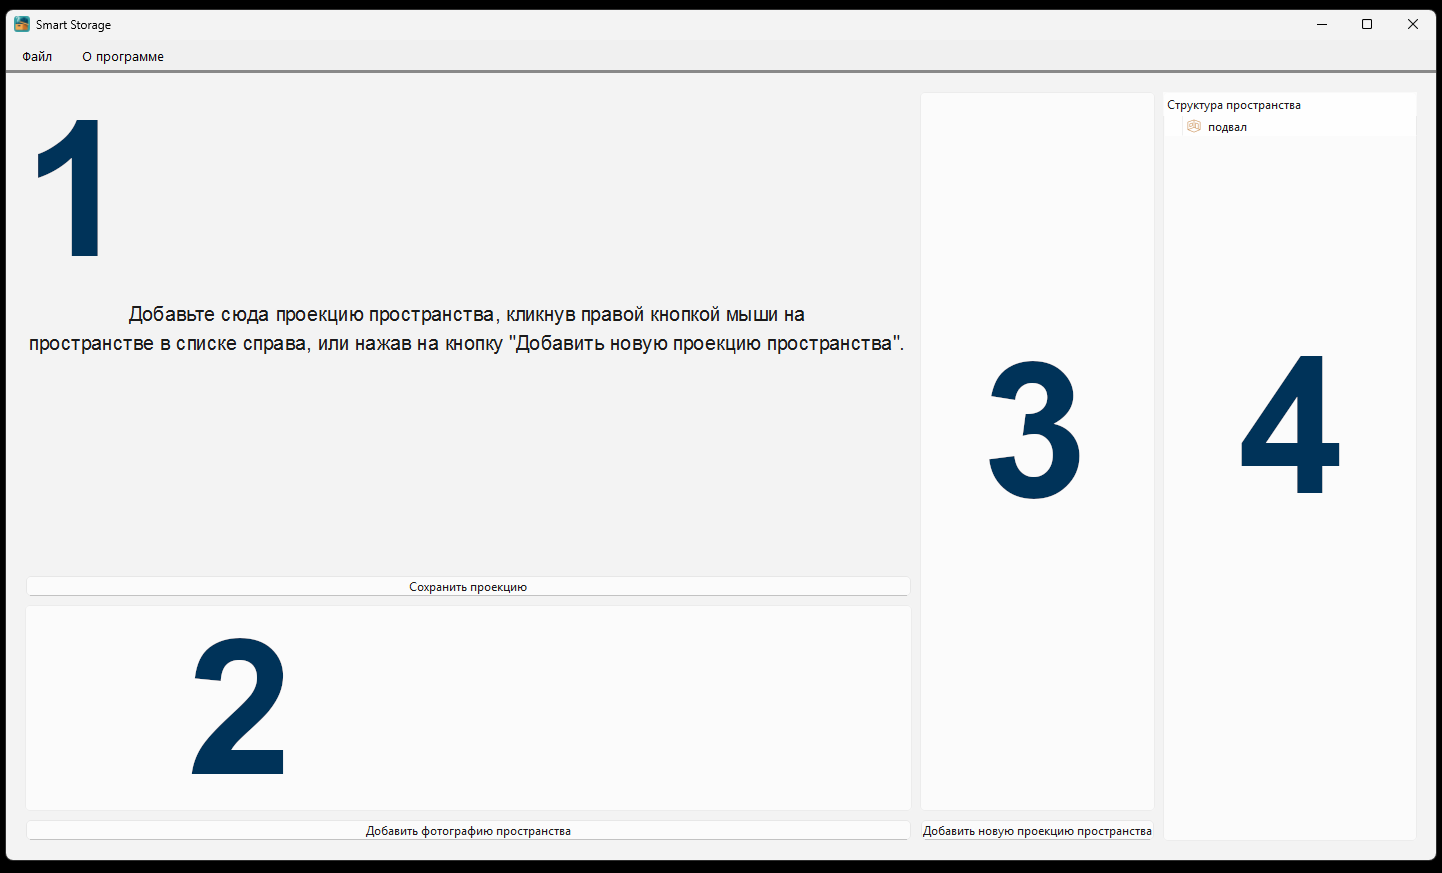
\includegraphics[width=0.9\textwidth]{images/space_added_with_numbers}
    \caption{Страница создания/редактирования пространства}
    \label{fig:space_added_with_numbers}
\end{figure}

\begin{enumerate}
    \item Поле для отображения 2D проекции пространства, с которой на данный момент работает пользлватель,
    \item Область, куда можно добавить фотографии или картинки, относящиеся к пространству,
    \item Тут пользователь может сохранить все развёртки пространства. Сохраненное состояние развертки, находящейся в работе, будет отображаться всегда на самом верху. Именно эти состояния развёрток будут сохраняться в базу данных при сохранении пространства,
    \item Здесь представлено дерево пространства. Корень дерева - это само пространство. У пространства может быть два типа узлов: подпространство и вещь. Данное дерево отображает только двойную вложенность. Это дерево предусмотрено для работы с развертками пространства и подразвертками вещей и подпространств пространства. Полный вид всей структуры соотношения пространств можно посмотреть выбрав пункт меню ``Файл'' $\rightarrow$ ``Показать всё дерево пространства''. Выбор этого пункта меню откроет дополнительный виджет, где будет показана вся структура, относящаяся к пространству, которое находится в работе. Пример этого виджета представлен на (рисунке~\ref{fig:full_space_structure}).

\begin{figure}[htbp]
    \centering
    \includegraphics[width=0.6\textwidth]{images/full_space_structure}
    \caption{Полная структура пространства.}
    \label{fig:full_space_structure}
\end{figure}

\end{enumerate}

\subsubsection{Создание проекций пространства}
Для загрузки изображения проекции пространства можно или выбрать соответствующий пункт (рисунок~\ref{fig:add_space_projection_context_menu}). из контекстного меню, которое появится при клике правой кнопкой мыши на имени пространства в структуре дерева справа или же нажав на кнопку ``Добавить новую проекцию пространства`` (рисунок~\ref{fig:button_add_new_space_projection}).

\begin{figure}[htbp]
    \centering
    \includegraphics[width=0.6\textwidth]{images/add_space_projection_context_menu}
    \caption{Вызов диалогового окна добавления проекции пространства из контекстного меню.}
    \label{fig:add_space_projection_context_menu}
\end{figure}

\begin{figure}[htbp]
    \centering
    \includegraphics[width=0.6\textwidth]{images/button_add_new_space_projection}
    \caption{Кнопка вызова диалогового окна добавления проекции пространства.}
    \label{fig:button_add_new_space_projection}
\end{figure}

При выборе одного из вариантов откроется диалоговое окно добавления проекции пространства (рисунок~\ref{fig:add_space_projection})
\begin{figure}[htbp]
    \centering
    \includegraphics[width=0.8\textwidth]{images/add_space_projection}
    \caption{Диалоговое окно добавления проекции пространства.}
    \label{fig:add_space_projection}
\end{figure}

В этом окне необходимо указать название проекции. В рамках проекций одного пространства, имена проекций должны быть уникальны. Необходимо загрузить картинку проекции пространства, а также указать её размеры в любых единицах измерения, которые выберет пользователь (метры, сантиметры, дюймы и т.д.) В дальнейшем необходимо придерживаться выбранной системы единиц измерения для подразверток подпространтсв и подразверток вещей для корректного отображения их размеров на развертке пространства. Для удобства пользователя, если соотношение сторон загружаемого изображения соответствует соотношению сторон реальной проекции пространства, можно отметить соответствующий чекбокс. После этого достаточно ввести длину проекции по одной стороне и нажать Enter — длина второй стороны проекции рассчитается автоматически. После нажатия OK проекция отобразится в соответствующем поле \gls{gui} (рисунок~\ref{fig:after_space_projection_addition})

\begin{figure}[htbp]
    \centering
    \includegraphics[width=0.8\textwidth]{images/after_space_projection_addition}
    \caption{Отображение проекции пространства, которая находится в работе.}
    \label{fig:after_space_projection_addition}
\end{figure}

В контекстном меню, выпадающем при нажатии правой кнопкой мыши на имя пространства, пункт ``Добавить проекцию пространства`` изменится на ``Изменить проекцию пространства`` (рисунок~\ref{fig:change_space_projection}). При выборе этого пункта меню появится диалоговое окно добавления проекции пространства с актуальными данными проекции, которая находится в работе. Можно будет изменить имя проекции, её описание, загрузить другое изображение или изменить размеры проекции. При этом, если на проекции пространтсва, уже имеются подпроекции подпространтсв пространтсва или подпроекции вещей пространтсва, то при изменеии размеров проекции пространства, подпроекции будут помещены в центр проекции пространтсва, так как при изменении размеров проекции, больше не известно в какой позиции должны находится подразвертки подпространств и вещей относительно развертки пространства. При изменении имени, описания или изображения проекции при сохранении её размеров позиции подпроекций относительно проекции будут сохранены.

\begin{figure}[htbp]
    \centering
    \includegraphics[width=0.8\textwidth]{images/change_space_projection}
    \caption{Изменить проекцию пространства}
    \label{fig:change_space_projection}
\end{figure}

При нажатии на кнопку ``Сохранить проекцию`` проекция будет сохранена как мини проекция (рисунок~\ref{fig:mini_projection}).
\begin{figure}[htbp]
    \centering
    \includegraphics[width=0.8\textwidth]{images/mini_projection}
    \caption{Сохраненная мини проекция проекции пространства}
    \label{fig:mini_projection}
\end{figure}

По кнопке ``Добавить новую проекцию пространства`` можно добавить сколько угодно проекций пространства. При их сохранении нажатием на кнопку ``Сохранить проекцию`` они будут сохранятся как мини проекции. При этом самой верхней мини проекцией будет отображаться та проекция, которая находится в работе, в её последнем сохраненном состоянии. При сохранении пространтсва именно те состояния проекций пространтсва, которые были сохранены как мини проекции, будут сохранены в базу данных. Пример большого количества сохраненных проекций пространства показан на (рисунке~\ref{fig:example_manz_mini_projections})

\begin{figure}[htbp]
    \centering
    \includegraphics[width=0.8\textwidth]{images/example_manz_mini_projections}
    \caption{Пример большого количества проекций пространства, сохраненных как мини проекции}
    \label{fig:example_manz_mini_projections}
\end{figure}

При клике правой кнопкой мыши по мини проекции появится контекстное меню (рисунок~\ref{fig:mini_projection_context_menu}). При выборе ``Открыть, как главную проекцию`` мини проекция отобразится слева и будет доступна для изменений. При выборе ``Удалить эту проекцию`` поведение будет различаться, в зависимости от того, относится ли контекстное меню к верхней мини проекции или к остальным мини проекциям. Если контекстное меню относится не к верхней мини проекции, то мини проекция будет просто удалена. Если же контекстное меню относится к верхней проекции, то будет выведено сообщение (рисунок~\ref{fig:remove_top_mini_projection_question}). Если будет выбран ответ Yes, то будет удалена мини проекция справа, а также удалена проекция слева, находящаяся в работе.
\begin{figure}[htbp]
    \centering
    \includegraphics[width=0.8\textwidth]{images/mini_projection_context_menu}
    \caption{Контекстное меню мини развертки}
    \label{fig:mini_projection_context_menu}
\end{figure}

\begin{figure}[htbp]
    \centering
    \includegraphics[width=0.8\textwidth]{images/remove_top_mini_projection_question}
    \caption{Контекстное меню мини развертки}
    \label{fig:remove_top_mini_projection_question}
\end{figure}

\subsubsection{Добавление подпространств и вещей в пространство}
\paragraph{Добавление вещей в пространство:}
Чтобы добавить вещь в пространство нужно выбрать в контекстном меню (рисунок~\ref{fig:add_space_projection_context_menu}) и  (рисунок~\ref{fig:change_space_projection})  ``Добавить вещь``. После этого откроется диалоговое окно (рисунок~\ref{fig:add_thing}). В нем необходимо в обязательном поле указать название вещи. Опционально можно добавить описание вещи, а также загрузить фотографии вещи. После того, как пользователь нажмёт ОК, то автоматически откроется диалоговое окно добавления проекции вещи. Пользователь может добавить проекцию вещи, указав имя проекции, загрузив картинку проекции и указав её размер в тех же единицах измерения, что проекция пространтсва, в которое добавляется вещь, а также опционально добавив описание проекции (рисунок~\ref{fig:add_thing_projection}). Пользователь может не добавлять проекцию вещи сразу, а добавить позже, выбрав пункт "Добавить развертку для вещи" в контекстном меню, выпадающем при щелчке правой кнопкой мыши на имени вещи в дереве справа (рисунок~\ref{fig:thing_context_menu}). После добавление вещи в пространство дерево справа будет автоматически обновлено - в нём появится имя добавленной вещи. Имена вещей в дереве расположены в алфавитном порядке.

\begin{figure}[htbp]
    \centering
    \includegraphics[width=0.8\textwidth]{images/add_thing}
    \caption{Диалоговое окно добавления вещи}
    \label{fig:add_thing}
\end{figure}

\begin{figure}[htbp]
    \centering
    \includegraphics[width=0.8\textwidth]{images/add_thing_projection}
    \caption{Диалоговое окно добавления проекции вещи}
    \label{fig:add_thing_projection}
\end{figure}

\begin{figure}[htbp]
    \centering
    \includegraphics[width=0.8\textwidth]{images/thing_context_menu}
    \caption{Контекстное меню вещи}
    \label{fig:thing_context_menu}
\end{figure}

После добавления проекции вещи она будет добавлена на проекцию пространтсва. В зависимости от прав пользователя (см. раздел~\ref{sec:users}), проекцию вещи можно перемещать в пределах непрозрачных областей изображения проекции пространства с помощью мыши или стрелками. Перемещаемая (выбранная) вещь будет подсвечена красным контуром (рисунок~\ref{fig:thing_projection_on_main_scene}). При нажатии на кнопку "Сохранить проекцию" проекция вещи будет сохранена на мини проекции пространства в той позиции, в которой она находится на проекции пространтсва слева в момент сохранения (рисунок~\ref{saved_thing_projection_on_mini_space_projection}).

\begin{figure}[htbp]
    \centering
    \includegraphics[width=0.8\textwidth]{images/thing_projection_on_main_scene}
    \caption{Проекция вещи на проекции пространтсва}
    \label{fig:thing_projection_on_main_scene}
\end{figure}

\begin{figure}[htbp]
    \centering
    \includegraphics[width=0.8\textwidth]{images/saved_thing_projection_on_mini_space_projection}
    \caption{Сохраненная проекция вещи на мини проекции пространтсва}
    \label{fig:saved_thing_projection_on_mini_space_projection}
\end{figure}

\paragraph{Добавление подпространств в пространство:} Чтобы добавить вещь в пространство нужно выбрать в контекстном меню (рисунок~\ref{fig:add_space_projection_context_menu}) и  (рисунок~\ref{fig:change_space_projection})  ``Добавить подпространство``. После этого откроется диалоговое окно (рисунок~\ref{fig:add_subspace}). Нужно указать имя подпространства и опционально описание подпространтсва.

\begin{figure}[htbp]
    \centering
    \includegraphics[width=0.8\textwidth]{images/add_subspace}
    \caption{Диалоговое окно добавления подпространтсва}
    \label{fig:add_subspace}
\end{figure}




\subsubsection{Добавление фотографий пространства}





\section{Пользователи}\label{sec:users}

\section*{Заключение}
Здесь подводятся итоги работы.

\begin{thebibliography}{9}
\bibitem{ref1} Автор. Название книги. Год.
\end{thebibliography}

\end{document}
